\documentclass{scrartcl}
\setkomafont{disposition}{\normalfont\bfseries}

\usepackage{fullpage}
\usepackage{tikz}
\usepackage[hang,flushmargin]{footmisc} 

\title{CS187 Assignment 4}
\subtitle{Finite-State Transducers}
\author{Lucas Freitas}
\date{\today}
\begin{document}

\setlength\parindent{0pt}
\maketitle

%% PROBLEM 1
\section*{Problem 1}
For all the items in the next pages, I used a Python script to generate a text file, which I then converted to \texttt{FST} format using:\\

\texttt{\$fstcompile --isymbols=test.sym --osymbols=test.sym --keep\_isymbols --keep\_osymbols --acceptor file.txt file.fst}\\

Where \texttt{file} is the name of each of the \texttt{FST} or text files. I then generated the PDF images of the automatons using the command:\\

\texttt{\$ fstdraw --isymbols=test.sym --osymbols=test.sym file.fst | dot -Tpdf > file.pdf}
\\
\subsection*{(1) Accept any letter in L (including space)}

To accept any letter in $L$, including space, we just need to create a Python script that outputs lines containing \texttt{0 1 letter} for each \texttt{letter} in $L$, so that any letter takes us to state  \texttt{1}, which we will be our final state.
\begin{verbatim}
# accept all alphabetical letters
for letter in string.ascii_uppercase + string.ascii_lowercase:
    file.write("0 1 %c\n" %letter)

# accept space
file.write("0 1 <spc>\n")
file.write("1")
\end{verbatim}
After compiling the text file (\texttt{p1a.txt}) with Open-FST, we generate the automaton below:
\begin{center}
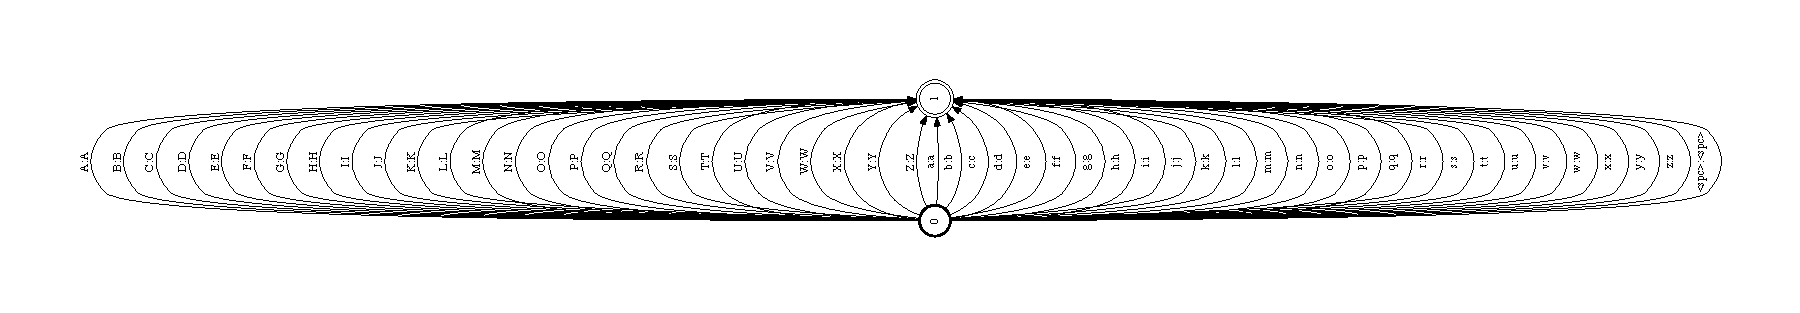
\includegraphics[width=170mm]{p1a.pdf}
\end{center}
\newpage
\subsection*{Problem 1.1 (Continued)}
Testing our automaton using \texttt{test-string.py}, we notice that the automaton seems to work properly (notice that the blank space below in the second test is actually a \texttt{<spc>}):
\begin{verbatim}
Please type a string to test: a
String is accepted
a

Please type a string to test:  
String is accepted
 
 
Please type a string to test: z
String is accepted
z

Please type a string to test: this shouldnt work
String is rejected
\end{verbatim}
\subsection*{(2) Accept a single space}
This automaton is even simpler. We just have to do the same as below, but only accepting the  \texttt{<spc>} letter instead of all possible letters in $L$.
\begin{verbatim}
# accept space
file.write("0 1 <spc>\n")
file.write("1")
\end{verbatim}
After compiling the text file (\texttt{p1b.txt}) with Open-FST, we generate the automaton below (a blank area of the PDF was cropped for better visualization):
\begin{center}
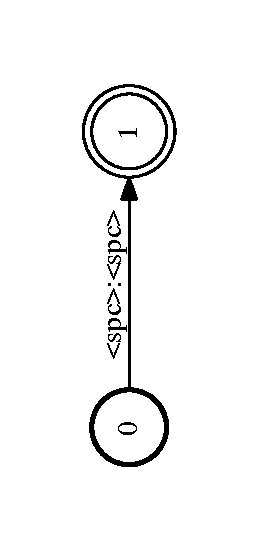
\includegraphics[width=20mm, angle=-90]{p1b.pdf}
\end{center}
Testing our automaton using \texttt{test-string.py}, we notice that the automaton seems to work properly (notice that the blank space below in the first test is actually a \texttt{<spc>}):
\begin{verbatim}
Please type a string to test:  
String is accepted
 
 
Please type a string to test: z
String is rejected

Please type a string to test: p
String is rejected

Please type a string to test: this shouldnt work
String is rejected
\end{verbatim}
\newpage
\subsection*{(3) Accept a capitalized word}
To accept a capitalized word, state \texttt{0} can only accept capital letters (\texttt{<spc>} not included), and should direct those to state \texttt{1}. No other letter should be accepted in state \texttt{0}. State \texttt{1} (the final state), on the other hand, should accept any lowercase letter (\texttt{<spc>} not included, as a word is defined in the specification as not having any space characters). The Python code to achieve that would be:
\begin{verbatim}
# accept first uppercase letter
    for letter in string.ascii_uppercase:
        file.write("0 1 %c\n" %letter)

# accepts following letters as lowercase
    for letter in string.ascii_lowercase:
        file.write("1 1 %c\n" %letter)
file.write("1")\end{verbatim}

After compiling the text file (\texttt{p1c.txt}) with Open-FST, we generate the automaton below (a blank area of the PDF was cropped for better visualization):
\begin{center}
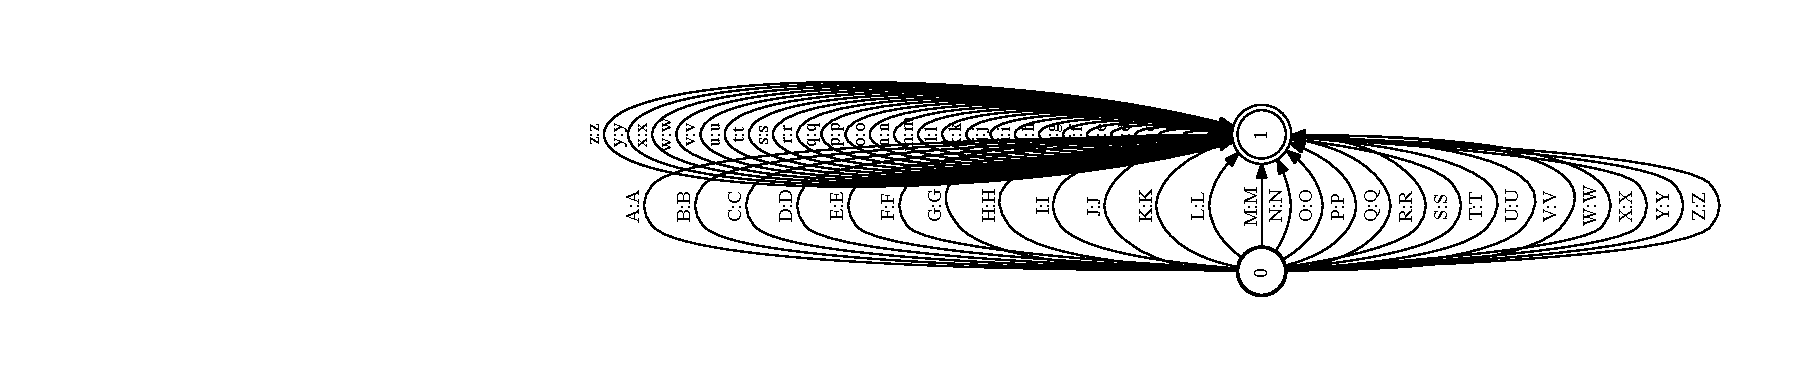
\includegraphics[width=160mm, angle=0]{p1c.pdf}
\end{center}
Testing our automaton using \texttt{test-string.py}, we notice that the automaton seems to work properly:
\begin{verbatim}
Please type a string to test: Schieber
String is accepted
Schieber

Please type a string to test: Csoneeightysevenisawesome
String is accepted
Csoneeightysevenisawesome

Please type a string to test: lucas
String is rejected

Please type a string to test: Lucas Freitas
String is rejected

Please type a string to test: turinG
String is rejected
\end{verbatim}
\newpage
\subsection*{(4) Accept a word containing the letter \texttt{a}}
To accept a word containing \texttt{a}, just accept any letter (except for  \texttt{<spc>}) in state \texttt{0}, directing all letters back to state  \texttt{0} except for  \texttt{a}, which should be directed to the final state \texttt{1}. State  \texttt{1} would then accept any letter except for  \texttt{<spc>}. The Python code to achieve that would be:
\begin{verbatim}
# loop non-a letters back to their current state
for letter in string.ascii_uppercase[1:] + string.ascii_lowercase[1:]:
    file.write("1 1 %c\n" %letter)
    file.write("0 0 %c\n" %letter)

# move a from state 0 to 1	
file.write("0 1 a\n")
file.write("1")
file.write("1")\end{verbatim}

After compiling the text file (\texttt{p1d.txt}) with Open-FST, we generate the automaton below (a blank area of the PDF was cropped for better visualization):\\
\begin{center}
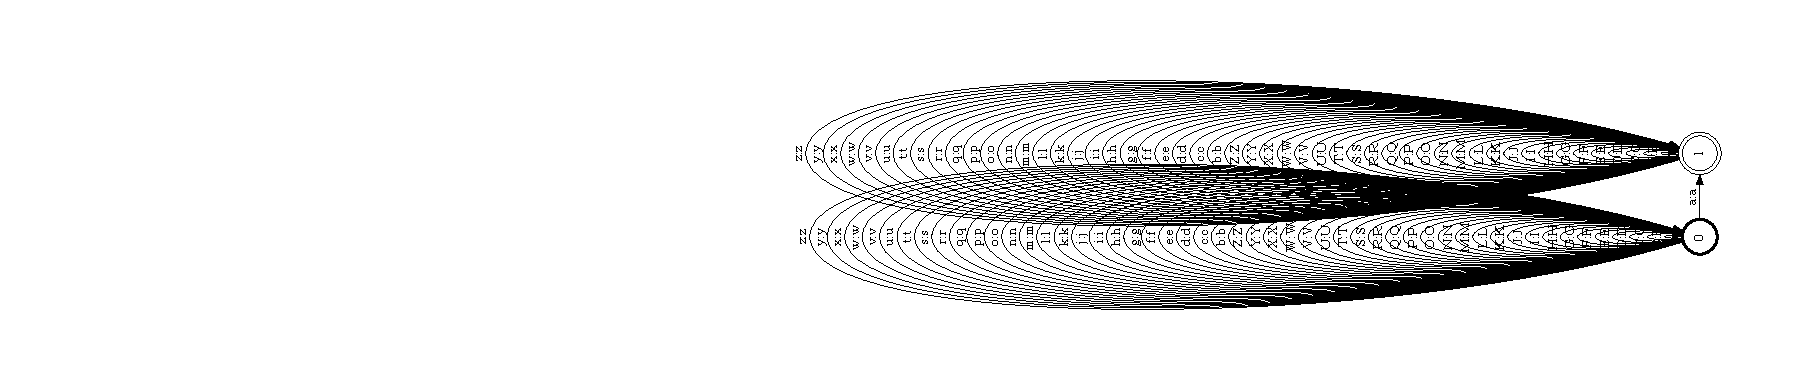
\includegraphics[width=140mm, angle=-0]{p1d.pdf}
\end{center}
Testing our automaton using \texttt{test-string.py}, we notice that the automaton seems to work properly:
\begin{verbatim}
Please type a string to test: lucas
String is accepted
lucas

Please type a string to test: lucAs
String is rejected

Please type a string to test: lucas freitas
String is rejected

Please type a string to test: csoneeightysevenisawesome
String is accepted
csoneeightysevenisawesome

Please type a string to test: csonesixtyonetoo
String is rejected
\end{verbatim}
\newpage

%% PROBLEM 2
\section*{Problem 2}
For all the items in the next pages, I used \texttt{FST} operations on the automatons from Problem 1 to generate a final automaton that achieves the function requested in the item. I then generated the PDF images of the automatons using the command:\\

\texttt{\$ fstdraw --isymbols=test.sym --osymbols=test.sym file.fst | dot -Tpdf > file.pdf}
\\
\subsection*{(1) Accept zero or more capitalized words followed by spaces}
For this case, we just need to accept both capitalized words or spaces. As said in Piazza, every accepted string should include a space as its last character, so the automaton should accept \texttt{Lucas<spc>Freitas<spc>}, but not \texttt{Lucas<spc>Freitas}.\\

To achieve that, we first need to concatenate the automatons from items \texttt{(3)} and \texttt{(2)} above, so that the resulting automaton will accept strings of the form \texttt{Word<spc>}, where \texttt{Word} is a capitalized string. Finally, we take the closure of the automaton, which will get us to accept a sequence of zero or more \texttt{Word<spc>}, i.e., capitalized words followed by spaces. The list of Open-FST operations to generate the final automaton is:
\begin{verbatim}
$ fstconcat p1c.fst p1b.fst > p2a_concat.fst
$ fstclosure p2a_concat.fst > p2a.fst
\end{verbatim}
The generated automaton can be seen below (a blank area of the PDF was cropped for better visualization):\\
\begin{center}
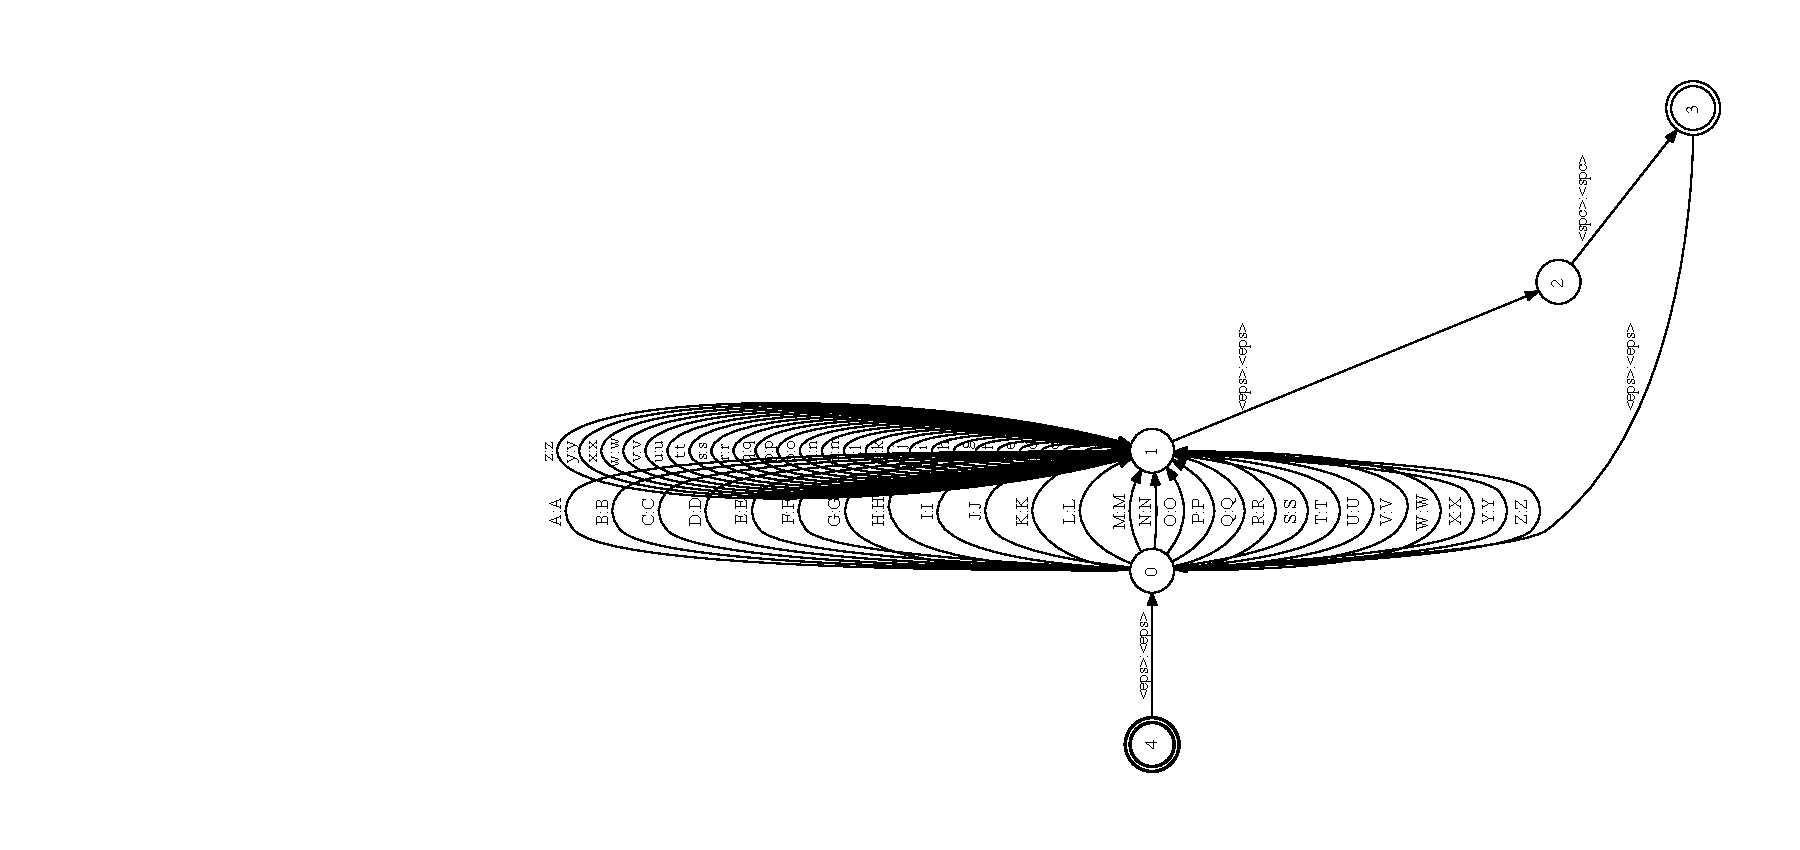
\includegraphics[width=160mm, angle=-0]{p2a.pdf}
\end{center}
\newpage
\subsection*{Problem 2.1 (Continued)}
Testing our automaton using \texttt{test-string.py}, we notice that the automaton seems to work properly (notice that in all examples besides the first, the string is ended with a space):
\begin{verbatim}
Please type a string to test: No Space At The End
String is rejected

Please type a string to test: Non capital Letter Somewhere
String is rejected

Please type a string to test: Lucas 
String is accepted
<eps>Lucas<eps> 

Please type a string to test: I Like This Class 
String is accepted
<eps>I<eps> <eps>Like<eps> <eps>This<eps> <eps>Class<eps> 
\end{verbatim}

\subsection*{(2) Accept a word beginning or ending in a capitalized letter}

As noted in Piazza, words might have capitalized letters at its beginning or end, but not in its middle. Therefore, we just have to realize that our final automaton should accept words that only start in a capitalized letter (capitalized word automaton from item \texttt{(3)} of Problem 1), words that only end in a capitalized letter (\texttt{fstreverse} of the capitalized word automaton), or both starts and ends with capitalized letter (\texttt{fstconcat} of the two previous automatons).\\

To achieve that, we just need to take the \texttt{fstunion} of the three automatons (take the \texttt{fstunion} of the first two, and then take the \texttt{fstunion} of the resulting automaton and of the third), since we want to accept any of the three kinds of strings. The list of Open-FST operations to generate the final automaton is:
\begin{verbatim}
$ fstreverse p1c.fst > p2b_reverse.fst
$ fstconcat p1c.fst p2b_reverse.fst > p2b_concat.fst
$ fstunion p1c.fst p2b_reverse.fst > p2b_temp.fst
$ fstunion p2b_temp.fst p2b_concat.fst > p2b.fst 
\end{verbatim}
The generated automaton can be seen below (a blank area of the PDF was cropped for better visualization):\\
\begin{center}
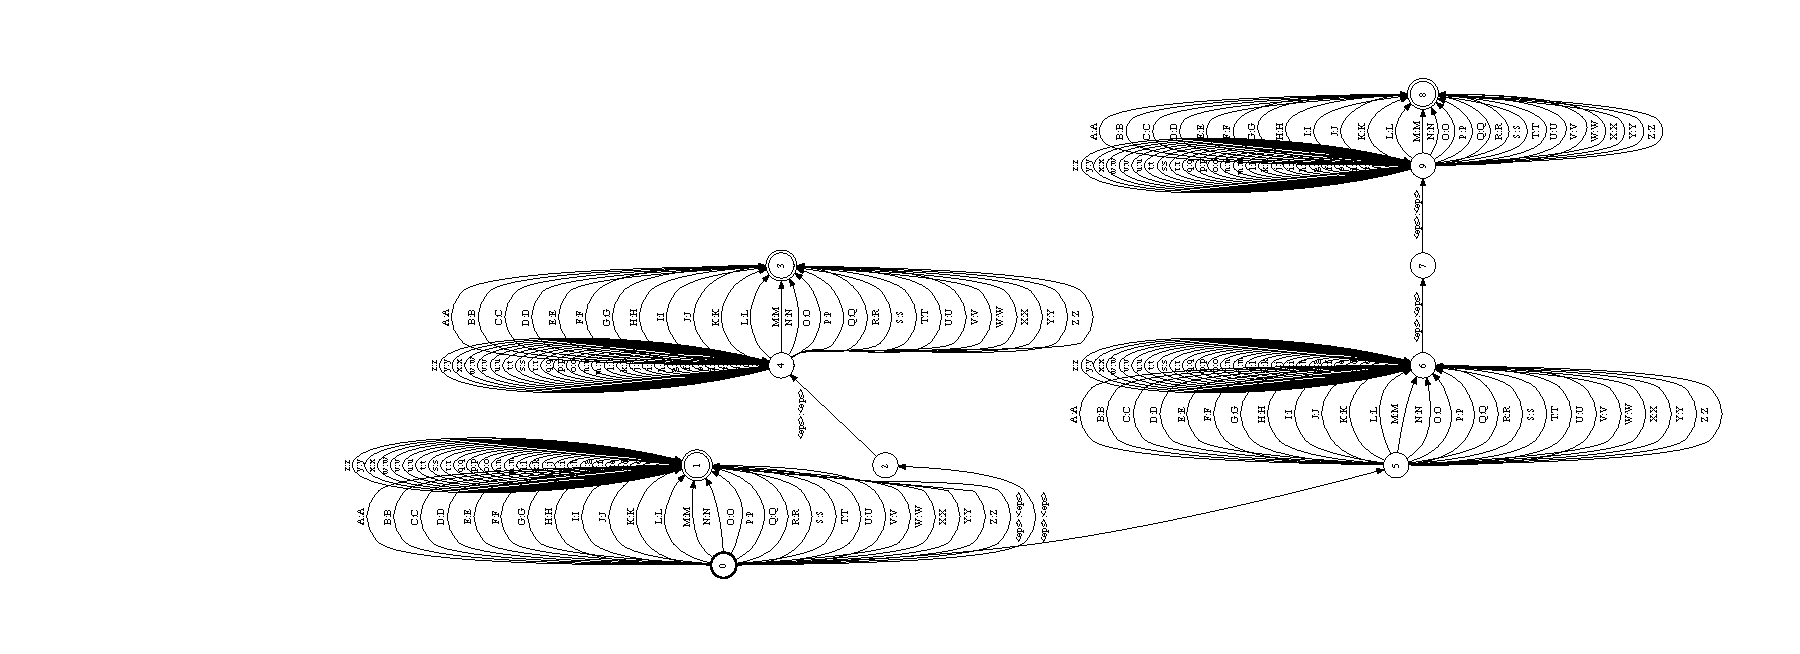
\includegraphics[width=141mm, angle=-0]{p2b.pdf}
\end{center}
\newpage
\subsection*{Problem 2.2 (Continued)}
Testing our automaton using \texttt{test-string.py}, we notice that the automaton seems to work properly (notice that for all examples besides the first, a space was added at the end of the string):
\begin{verbatim}
Please type a string to test: Chinese
String is accepted
Chinese

Please type a string to test: persiaN
String is accepted
<eps><eps>persiaN

Please type a string to test: JapanesE
String is accepted
<eps>J<eps><eps>apanesE
\end{verbatim}

\begin{verbatim}
Please type a string to test: PorTuguesE
String is rejected
\end{verbatim}

\subsection*{Note (additional automaton)}
If we want to also accept words that  begin or end in a capitalized letter, and might also have capitalized letter in their middle, one thing that we can is generate an automaton (let's call is \texttt{A}) that represents a generic word with any letters in $L$ (\texttt{<spc>} not included), and make concatenations of \texttt{A} and the capitalized word automaton, the reverse capitalized word automaton and \texttt{A}, and the capitalized word automaton, \texttt{A}, and the reverse capitalized word automaton.\\

Taking the union of the three concatenations will generate the automaton we are looking for. To generate \texttt{A}, we just need to take the difference of the automatons in items \texttt{(1)} and \texttt{(2)} from Problem 1, and then take the \texttt{fstclosure} of the generated automaton. The list of Open-FST operations to generate the final automaton is:
\begin{verbatim}
$ fstdifference p1a.fst p1b.fst > p2b_letters.fst
$ fstclosure p2b_letters.fst > p2b_words.fst
$ fstreverse p1c.fst > p1c_reverse.fst
$ fstconcat p1c.fst p2b_words.fst > p2b_begincap.fst
$ fstconcat p2b_words.fst p1c_reverse.fst > p2b_endcap.fst
$ fstconcat p2b_begincap.fst p1c_reverse.fst > p2b_bothcap.fst
$ fstunion p2b_begincap.fst p2b_endcap.fst > p2b_tempunion.fst
$ fstunion p2b_tempunion.fst p2b_bothcap.fst > p2b_note.fst
\end{verbatim}
\newpage
\subsection*{Problem 2.2 (Continued)}
The generated automaton can be seen below (a blank area of the PDF was cropped for better visualization):
\begin{center}
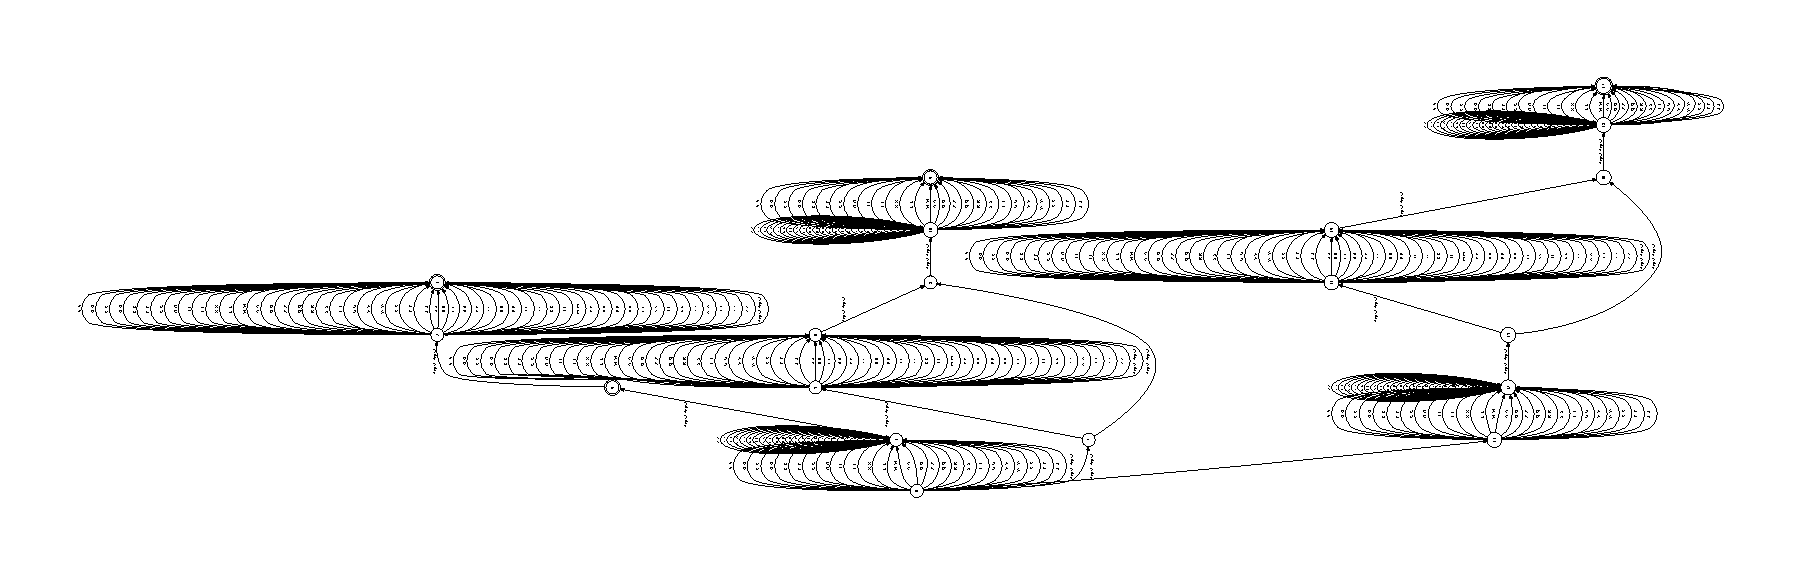
\includegraphics[width=165mm, angle=-0]{p2b_note.pdf}
\end{center}
Testing our automaton using \texttt{test-string.py}, we notice that the automaton seems to work properly (notice that for all examples besides the first, a space was added at the end of the string):
\begin{verbatim}
Please type a string to test: Lucas
String is accepted
L<eps><eps>u<eps>c<eps>a<eps>s

Please type a string to test: lucaD
String is accepted
<eps><eps><eps>lucaD

Please type a string to test: LucaS
String is accepted
<eps>L<eps><eps><eps>ucaS

Please type a string to test: LuCaS
String is accepted
<eps>L<eps><eps>u<eps>C<eps><eps>aS

Please type a string to test: lucAs
String is rejected

Please type a string to test: lucas
String is rejected
\end{verbatim}

\subsection*{(3) Accept a word that is capitalized and contains the letter \texttt{a}}
For this item, we just need to take the intersection of the automatons from items \texttt{(3)} and \texttt{(4)} in Problem 1, since we want the word to be both capitalized and to contain the letter \texttt{a}. The Open-FST operation to generate the final automaton is:
\begin{verbatim}
$ fstintersect p1c.fst p1d.fst > p2c.fst
\end{verbatim}
\newpage
\subsection*{Problem 2.3 (Continued)}
The generated automaton can be seen below (a blank area of the PDF was cropped for better visualization):\\
\begin{center}
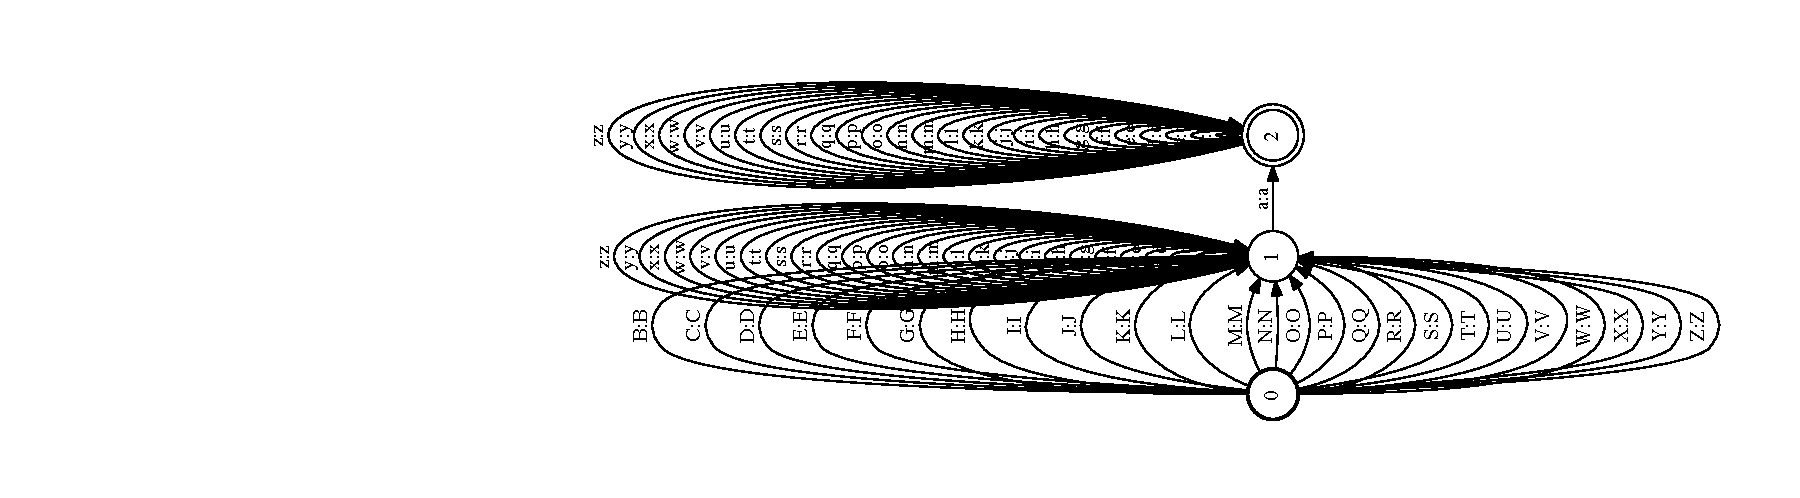
\includegraphics[width=170mm, angle=-0]{p2c.pdf}
\end{center}
Testing our automaton using \texttt{test-string.py}, we notice that the automaton seems to work properly (notice that for all examples besides the first, a space was added at the end of the string):
\begin{verbatim}
Please type a string to test: Lucas
String is accepted
Lucas

Please type a string to test: Scheiber
String is rejected

Please type a string to test: allen
String is rejected

Please type a string to test: Harry Potter
String is rejected
\end{verbatim}
\subsection*{(4) Accept a word that is capitalized or does not contain an \texttt{a}}
For this last item, we just need to take the union of the automaton from item \texttt{(3)} of Problem 1 and the negation of item \texttt{(4)} of Problem 1, which can be calculated from the \texttt{fstdifference} of all the words with letters in L (\texttt{<spc>} not included) and item \texttt{(4)}, since we want the word to be capitalized or to not contain the letter \texttt{a} (negation of containing letter \texttt{a}). The Open-FST operation to generate the final automaton is (notice that we had to sort arcs to fulfill the requirements of \texttt{fstdifference}):

\begin{verbatim}
$ fstdifference p1a.fst p1b.fst > p2b_letters.fst
$ fstclosure p2b_letters.fst > p2b_words.fst
$ fstarcsort p1d.fst > sorted_p1d.fst
$ fstdifference p2b_words.fst sorted_p1d.fst > not_a.fst
$ fstunion p1c.fst not_a.fst > p2d.fst
\end{verbatim}
\newpage
\subsection*{Problem 2.4 (Continued)}
The generated automaton can be seen below (a blank area of the PDF was cropped for better visualization):
\begin{center}
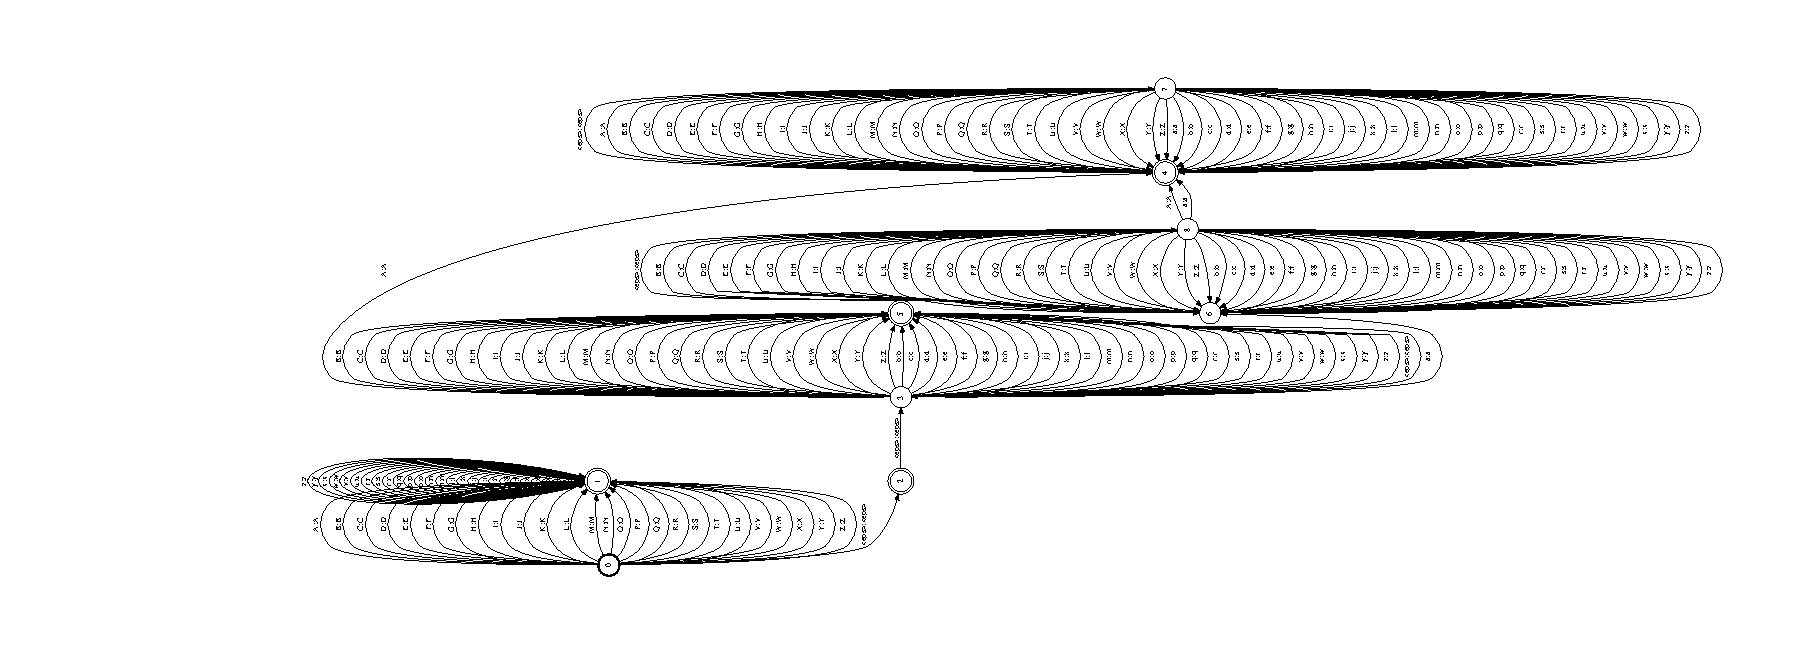
\includegraphics[width=160mm, angle=-0]{p2d.pdf}
\end{center}
Testing our automaton using \texttt{test-string.py}, we notice that the automaton seems to work properly (notice that for all examples besides the first, a space was added at the end of the string):
\begin{verbatim}
Please type a string to test: Lucas
String is accepted
Lucas

Please type a string to test: Schieber
String is accepted
<eps><eps>S<eps>c<eps>h<eps>i<eps>e<eps>b<eps>e<eps>r

Please type a string to test: lucas
String is rejected

Please type a string to test: schieber
String is accepted
<eps><eps>s<eps>c<eps>h<eps>i<eps>e<eps>b<eps>e<eps>r
\end{verbatim}
\subsection*{(5) Solve the previous item without using \texttt{fstunion}}
Accepting a word that is capitalized or does not contain an \texttt{a} is the same as accepting all words with any letters in L (except for \texttt{<spc>}) except for those that are both not capitalized and contain the letter \texttt{a}.\\

To accept words that are both uncapitalized and contain the letter \texttt{a}, first we have to take the \texttt{fstdifference} of all possible words and capitalized words (generating automaton \texttt{X}, which accepts uncapitalized words), and then take the \texttt{fstdifference} of all possible words and all words containing \texttt{a} (generating automaton \texttt{Y}, which accepts words without \texttt{a}).\\

We then take the \texttt{fstdifference} of \texttt{X} and \texttt{Y}, generating an automaton \texttt{Z} that accepts uncapitalized words that contain the letter \texttt{a}. Finally, we take the \texttt{fstdifference} of all possible words and \texttt{Z}, and our desired automaton should be generated.\\

Luckily enough, we have already generated an automaton for all possible words in the note for item \texttt{2}, so the list of Open-FST operations we need to perform is:
\begin{verbatim}
$ fstdifference p1a.fst p1b.fst > p2b_letters.fst
$ fstclosure p2b_letters.fst > p2b_words.fst
$ fstdifference p2b_words.fst p1c.fst > uncap.fst
$ fstarcsort p1d.fst > sorted_p1d.fst
$ fstdifference p2b_words.fst sorted_p1d.fst > not_a.fst
$ fstrmepsilon not_a.fst > no_epsilon_or_a.fst
$ fstarcsort no_epsilon_or_a.fst > sorted_no_a.fst
$ fstdifference uncap.fst sorted_no_a.fst > almost_there.fst
$ fstrmepsilon almost_there.fst > no_epsilon_almost_there.fst
$ fstarcsort no_epsilon_almost_there.fst > arcsort_there.fst
$ fstdifference p2b_words.fst arcsort_there.fst > p2e.fst

\end{verbatim}
Notice that we had to remove epsilons and sort arcs to fulfill the requirement of some of the methods. Let's see what the automaton looks like! The generated (and super cool) automaton can be seen below (a blank area of the PDF was cropped for better visualization):
\begin{center}
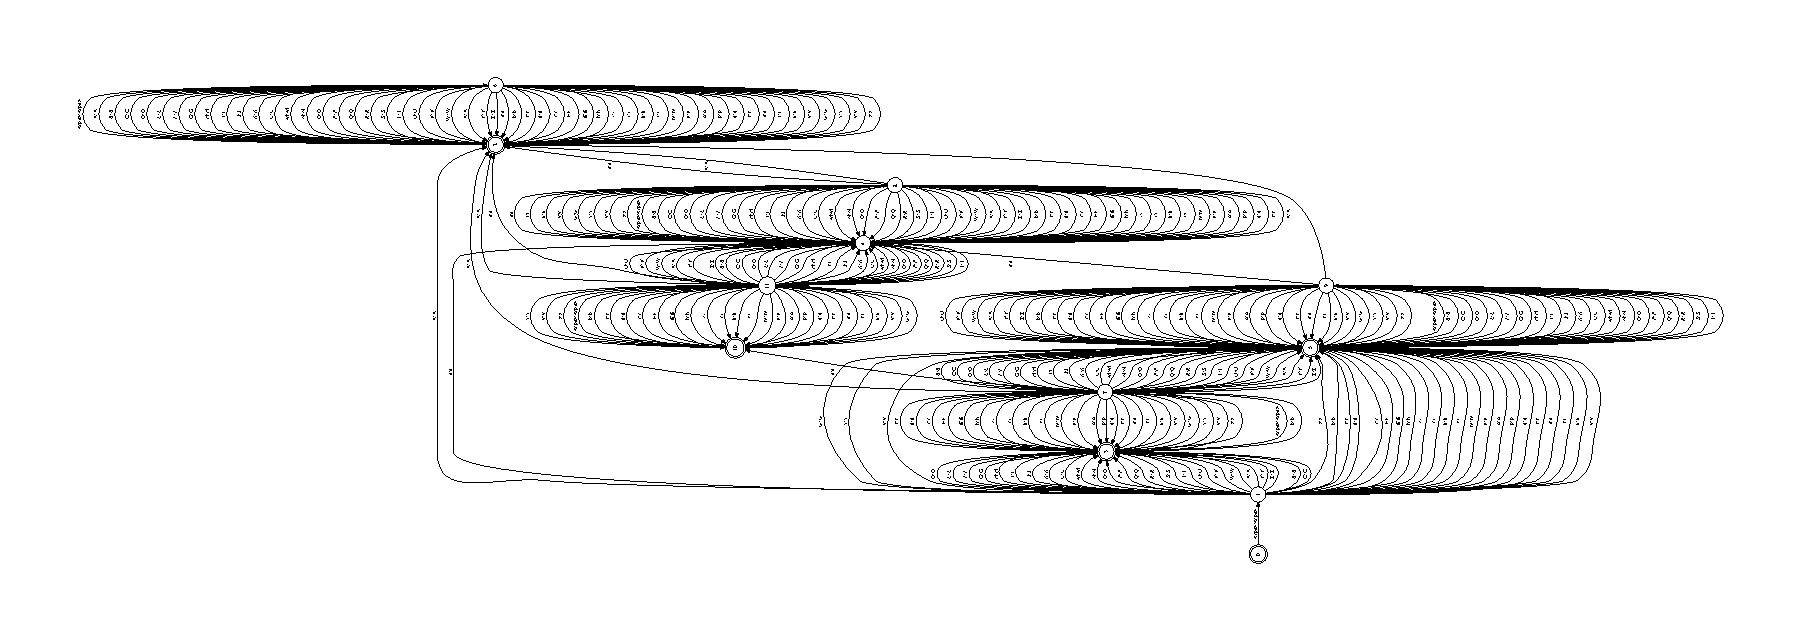
\includegraphics[width=170mm, angle=-0]{p2e.pdf}
\end{center}
Testing our automaton using \texttt{test-string.py}, we notice that the automaton seems to work properly (notice that for all examples besides the first, a space was added at the end of the string):
\begin{verbatim}
Please type a string to test: Lucas
String is accepted
<eps>L<eps>u<eps>c<eps>a<eps>s

Please type a string to test: Schieber
String is accepted
<eps>S<eps>c<eps>h<eps>i<eps>e<eps>b<eps>e<eps>r
\end{verbatim}
\newpage
\subsection*{Problem 2.5 (Continued)}
\begin{verbatim}
Please type a string to test: lucas
String is rejected

Please type a string to test: schieber
String is accepted
<eps>s<eps>c<eps>h<eps>i<eps>e<eps>b<eps>e<eps>r
\end{verbatim}

\newpage
%% PROBLEM 3
\section*{Problem 3}
\subsection*{(1) How many states cat be reached from the initial state?}
Only two states can be reached: \texttt{1} and \texttt{2}.

\subsection*{(2) How many states can reach a final state?}
States \texttt{0}, \texttt{3}, and \texttt{4} can reach a final state. As an example, the state \texttt{0} can reach the final state \texttt{2} by getting \texttt{2} as input, while the state \texttt{3} can reach the final state \texttt{4} if it gets the input \texttt{4}. Finally, the final state \texttt{4} can reach the final state \texttt{4} (itself) by receiving the string \texttt{34} as input.
\subsection*{(3) Compile the automaton and use OpenFTS to remove all useless states}
We can compile the automaton by creating a \texttt{.sym} file for \texttt{isymbols} and \texttt{osymbols} as the one below (the file can be found in the submission folder as \texttt{p3.sym}):
\begin{verbatim}
1 1
2 2
3 3
4 4
\end{verbatim}
Using the automaton given and running the commands below, we obtain the following automaton:\\

\texttt{\$ fstcompile --isymbols=p3.sym --osymbols=p3.sym --keep\_isymbols --keep\_osymbols --acceptor p3.txt p3.fst}\\

\texttt{\$ fstdraw --isymbols=test.sym --osymbols=test.sym file.fst | dot -Tpdf > file.pdf}
\\
\begin{center}
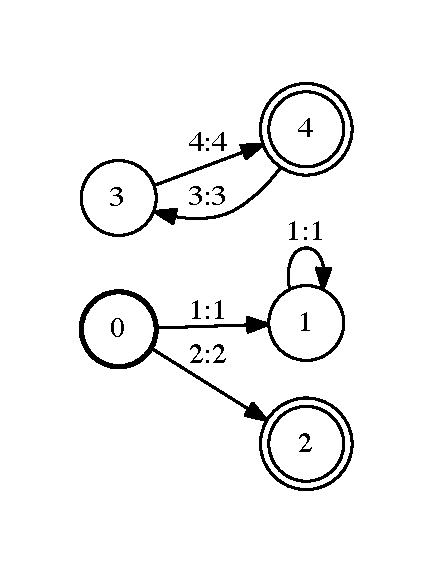
\includegraphics[width=25mm, angle=-0]{p3.pdf}
\end{center}
We can remove the useless states by running:\\

\texttt{\$ fstconnect p3.fst p3\_new.fst}\\

And then draw the new automaton by running:\\

\texttt{\$ fstdraw --isymbols=p3.sym --osymbols=p3.sym p3\_new.fst | dot -Tpdf > p3\_new.pdf}\\

The resultant automaton can be seen below:
\begin{center}
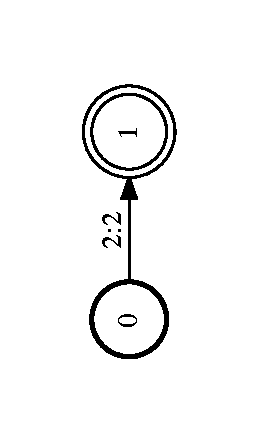
\includegraphics[width=10mm, angle=-90]{p3_new.pdf}
\end{center}
\newpage

%% PROBLEM 4
\section*{Problem 4}
\subsection*{(1) Create a transducer that implements the \texttt{rot13} cipher}

To implement the \texttt{rot13} cipher, all we have to do is rotate lowercase letters $13$ positions in the alphabet, while leaving the space unchanged. That way, the transducer will only have one state, and will accept any lowercase letter or space. The text file (\texttt{p4.txt}) can be generated from the Python script below:
\begin{verbatim}
letters = string.ascii_lowercase

# encode message
for i in range(26):
    file.write("0 0 %c %c\n" %(letters[i], letters[(i + 13) % 26]))
	
# space encodes to space
file.write("0 0 <spc> <spc>\n")
file.write("0")
\end{verbatim}
After compiling the text file (\texttt{p4.txt}) with Open-FST, we generate the automaton below (a blank area of the PDF was cropped for better visualization):

\begin{center}

\includegraphics[width=150mm]{p4.pdf}
\end{center}

\subsection*{(2) Encode and decode the message given}
To encode and decode the message, we can just run \texttt{\$ python test-string.py} inputting each of the messages, as in the items below:
\itemize
\item
Encode \texttt{how many yale students does it take to change a lightbulb} (the encoded message is the last line of output):
\begin{verbatim}
Please type a string to test: how many yale students does it take to change a lightbulb
String is accepted

ubj znal lnyr fghqragf qbrf vg gnxr gb punatr n yvtugohyo
\end{verbatim}

\item
Decode \texttt{abar arj unira ybbxf orggre va gur qnex�} (the decoded message is the last line of output):
\begin{verbatim}
Please type a string to test: abar arj unira ybbxf orggre va gur qnex
String is accepted

none new haven looks better in the dark
\end{verbatim}

\end{document}